\mode<presentation>
{
  \usetheme{Boadilla}
}

\usepackage[utf8]{inputenc}
\usepackage{booktabs}

\usepackage{minted}
%\usepackage[draft]{minted}
\setminted{frame=single}

\title{Empathy}
\subtitle{With an emphasis on the tech community}
\author{Franklin Chen \\ \url{http://franklinchen.com/}}
\institute{\href{http://www.codeandsupply.co/}{Pittsburgh Code and Supply}}
\date[April 15, 2015]{\href{http://www.meetup.com/Pittsburgh-Code-Supply/events/221553015/}{April 15, 2015}}

\subject{Talks}

\AtBeginSection[]
{
  \begin{frame}<beamer>{Outline}
    \tableofcontents[currentsection,subsectionstyle=hide]
  \end{frame}
}

\begin{document}

\maketitle

\begin{abstract}
I've been in the tech world for over twenty years now, since my first job as a software engineer in 1993. In recent years, I have come to believe that people skills as well as technical skills are necessary for all of us, especially with the increasingly fast pace in the tech world and the involvement of many stakeholders. One thing I've been working on myself, and hope to see more of in our world, is empathy.

I would like to give an overview of what empathy is, what it is not, different kinds of empathy, possible pitfalls, and concrete ways we can improve how our tech communities operate, by understanding our human nature. I will share examples of difficult scenarios I have experienced or actively participated in, where empathy could have made the situations less negative.
\end{abstract}

\begin{frame}
  \titlepage{}
\end{frame}

\section*{Outline}

\begin{frame}{Outline}
  \tableofcontents[subsectionstyle=hide]
\end{frame}

\section{Why this talk?}

\subsection{I almost quit the tech community in 2014}

\begin{frame}{I almost quit the tech community in 2014}
  \begin{block}{Paradox in 2014}
    \begin{itemize}
    \item \emph{Locally}: many good things happening
    \item \emph{Globally}: many bad things I saw online
    \item \emph{Personally}: doubts about my own direction
    \end{itemize}
  \end{block}

  \begin{alertblock}{Not my first moment of doubt}
    I have quit the tech community before: 1999--2009
  \end{alertblock}

  \begin{block}{December 2014}
    \begin{itemize}
    \item Identified the core problem: lack of \emph{empathy}
    \item Decided to change my life
    \item Proposed this talk topic for Pittsburgh Code and Supply
    \end{itemize}
  \end{block}
\end{frame}

\begin{frame}{What happened in 2014?}
  \begin{block}{What I saw online}
    \begin{itemize}
    \item Discourse got worse: Twitter, Reddit, mailing lists,
      etc.
    \item Not just tech, but especially tech: people talking past each
      other, yelling
    \item Realized I'm part of the problem too
    \end{itemize}
  \end{block}

  \begin{block}{I felt dissonance with my mission}
    \begin{itemize}
    \item Teaching
    \item Learning
    \item Sharing
    \item Actually being helpful
    \end{itemize}
  \end{block}
\end{frame}

\begin{frame}{Stepping away}
  \begin{block}{Changes I've made}
    \begin{itemize}
    \item I changed how I behave online
    \item I temporarily stopped writing for my three blogs
      \begin{itemize}
      \item Not satisfied with my old writings
      \end{itemize}
    \item I changed my focus in my side projects, to incorporate more empathy
    \end{itemize}
  \end{block}
\end{frame}


\section{What empathy is (and isn't)}

\begin{frame}{Good book on empathy}
  \begin{figure}
    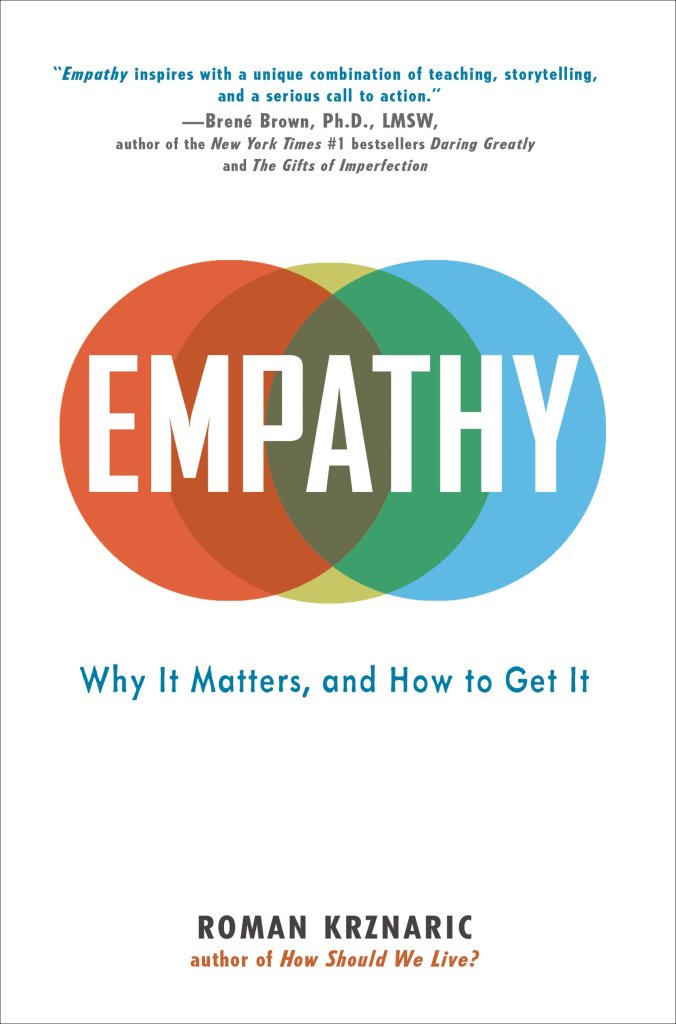
\includegraphics[width=0.25\textwidth]{Empathy-USA-cover-low-res-676x1024.jpg}
  \end{figure}

  \href{http://www.romankrznaric.com/}{Roman Krznaric}: {\emph{Empathy: Why It
        Matters, and How to Get It}}
\end{frame}

\subsection{What empathy isn't}

\begin{frame}{What empathy isn't}
  \begin{block}{Empathy is \emph{not}:}
    \begin{itemize}
    \item Fuzzy, feel-good sentiment
    \item Being tender and caring toward others
    \item Sympathy, feeling sorry for someone
    \item Charity, self-sacrifice
    \item Compassion
    \end{itemize}
  \end{block}
\end{frame}

\begin{frame}{Especially: not the Golden Rule}
  \begin{block}{Golden Rule}
    ``Do unto others as you would have them do unto you''
  \end{block}
\end{frame}


\subsection{What empathy is}

\begin{frame}{What empathy is}
  \begin{block}{Empathy is:}
    ``The art of stepping \emph{imaginatively} into the shoes of
    another person, \emph{understanding} their \emph{feelings} and
    \emph{perspectives}, and using that understanding to guide your
    \emph{actions}''
  \end{block}
\end{frame}

\begin{frame}{Imagination}
  \begin{itemize}
  \item Requires conscious effort
  \item It's hard!
  \item It can be intriguing
  \item It can be unsettling, make you feel vulnerable
  \end{itemize}
\end{frame}

\begin{frame}{Empathy even for enemies?}
  \begin{figure}
    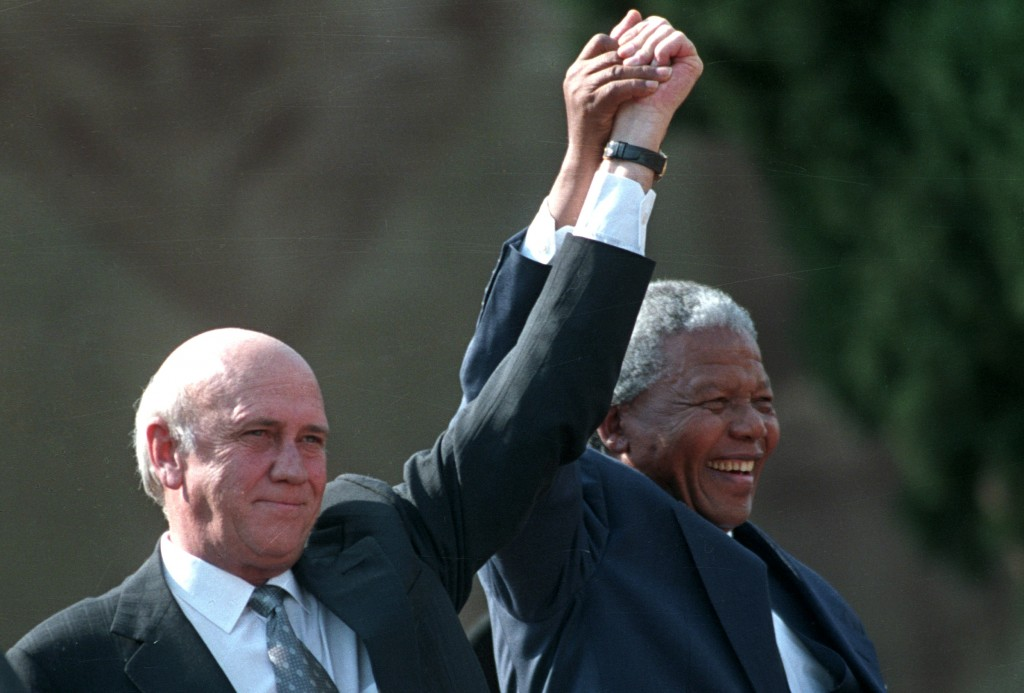
\includegraphics[width=0.5\textwidth]{deklerk-mandela1-1024x693.jpg}
  \end{figure}

  Nelson Mandela and de Klerk

  (Photo from \href{http://blogs.reuters.com/great-debate/2013/12/09/mandela-and-de-klerk-essential-partners/}{Reuters})
\end{frame}

\begin{frame}{The two halves of empathic understanding}
  \begin{description}
  \item[Affective] ``emotional'' side
  \item[Cognitive] ``rational'' side (\href{http://en.wikipedia.org/wiki/Perspective-Taking}{``perspective-taking''})
  \end{description}

\end{frame}

\begin{frame}{Cognitive empathy}
  \begin{figure}
    
\includegraphics[width=0.25\textwidth]{Mastermind-cover-new-pipe.jpg}
  \end{figure}

  \href{http://aeon.co/magazine/psychology/maria-konnikova-empathy-sherlock-holmes/}{Sherlock
    Holmes}, strategic about understanding people.
\end{frame}

\begin{frame}{Both halves are needed}
  A sociopath can
  \begin{itemize}
  \item Understand you very well
  \item But not care about your well-being
  \end{itemize}
\end{frame}

\begin{frame}{Back to the Golden Rule}
  Is there an alternative to the Golden Rule?
\end{frame}

\begin{frame}{The Platinum Rule}
  \begin{block}{Platinum Rule}
    ``Do unto others as they would have you do unto them''
  \end{block}

  People are different from you.
  \begin{itemize}
  \item Different values
  \item Different interests
  \item Different goals
  \end{itemize}

  A true test of empathy: \href{http://www.progressiveimpact.org/a-true-test-of-empathy-towards-others/}{when you might have something to lose}
\end{frame}

% TODO extraneous?
%\begin{frame}{Example: pro versus amateur culture and standards}
%  \begin{figure}
%    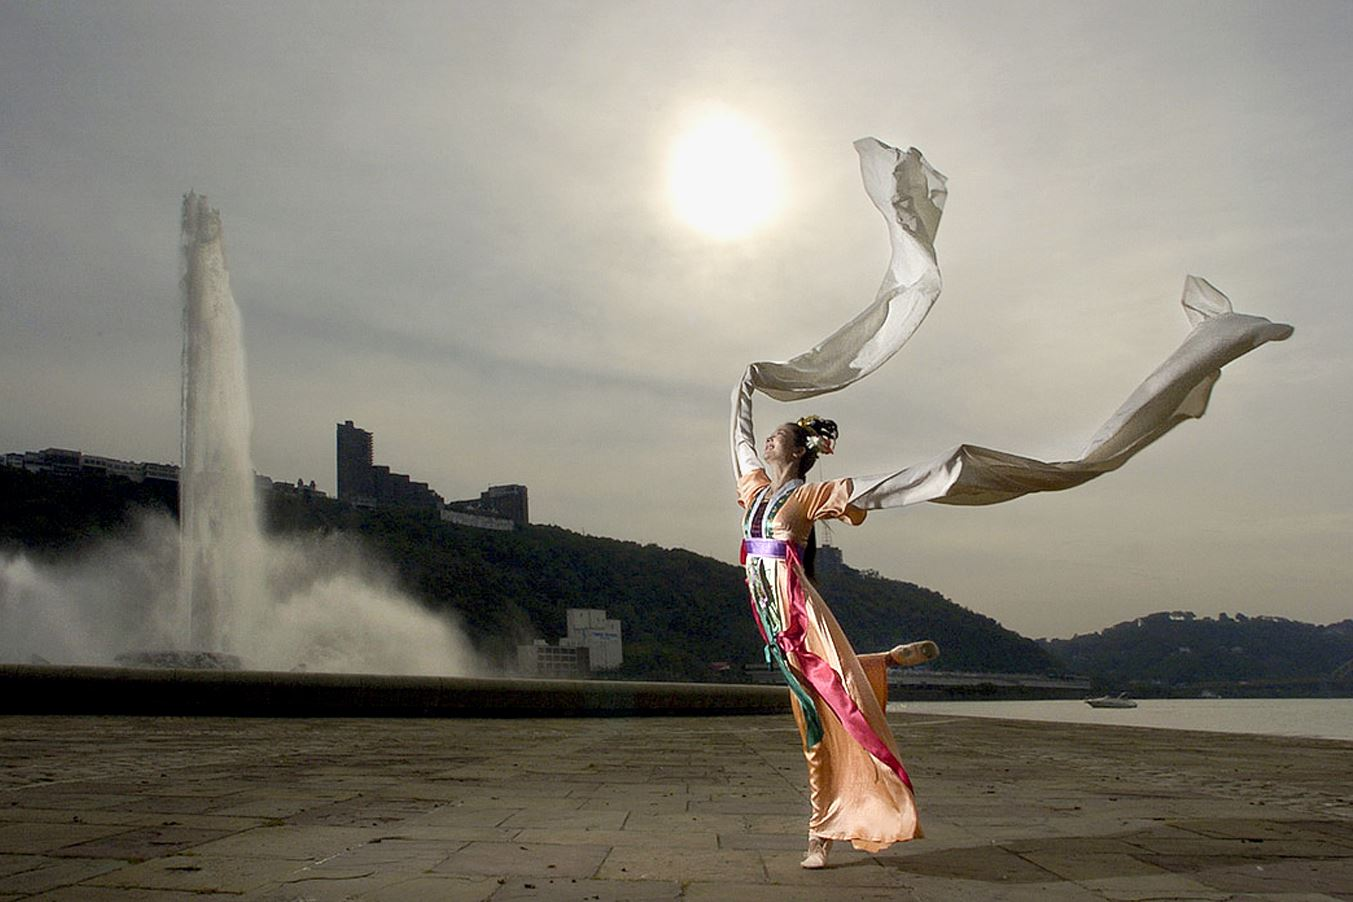
\includegraphics[width=0.5\textwidth]{Odysseys-China.jpg}
%  \end{figure}
%
%  Yanlai Wu, dance instructor,
%  \href{http://www.post-gazette.com/newimmigrants/2015/04/13/Odysseys-Teaching-the-grace-of-Chinese-dancing-brought-her-to-Pittsburgh/stories/201504130032}{immigrant
%    to Pittsburgh}, had to modify her teaching
%\end{frame}

\begin{frame}{``Empathic dissent''}
  \begin{itemize}
  \item Empathy doesn't mean agreement
  \item It means understanding
  \end{itemize}

  ``I have no idea why they would do/think that!'': a starting point,
  not a dead end
\end{frame}

\begin{frame}{Self-empathy}
  Put yourself in your own shoes too!
\end{frame}

\section{Examples of empathy (or not) in my career}

\subsection{Learning computer science, programming}

\begin{frame}{My first computing experiences}
  Middle school:
  \begin{itemize}
  \item 6th grade: forced by math teacher to stay after school and
    learn BASIC and program TRS-80
  \item Teacher used wrong filter for who would be interested!
  \end{itemize}

  High school:
  \begin{itemize}
  \item 9th grade: ``computer literacy'' credit required, took COBOL,
    almost failed
  \item School requirements inflexible
  \end{itemize}
\end{frame}

\begin{frame}{Why I quit computer programming after high school}
  High school:
  \begin{itemize}
  \item 11th grade: Advanced Placement Computer Science (1985, Pascal)
    \begin{itemize}
    \item Took in order to never have to code again!!
    \end{itemize}
  \item A classmate named all his variables four-letter words
    \begin{itemize}
    \item I felt bad for the teacher but didn't say anything
    \end{itemize}
  \item Long nights of debugging
    \begin{itemize}
    \item Development environments were, and still are,
      \href{https://vimeo.com/115154289}{inhumane} (Bret Victor)
    \end{itemize}
  \end{itemize}

  College:
  \begin{itemize}
  \item (Was physics major)
  \item Failed freshman week BASIC programming exam (had to learn enough
    \texttt{vi} and Unix)
  \item Computing culture turned me off
    \begin{itemize}
    \item Weed-out classes, much bragging
    \end{itemize}
  \item Consequence: no computer programming in college
  \end{itemize}
\end{frame}


\begin{frame}{Women in computing}
  30 years later, still \href{http://www.aauw.org/2015/03/11/is-computing-just-for-men/
}{problems attracting women in the US}!

  \begin{figure}
    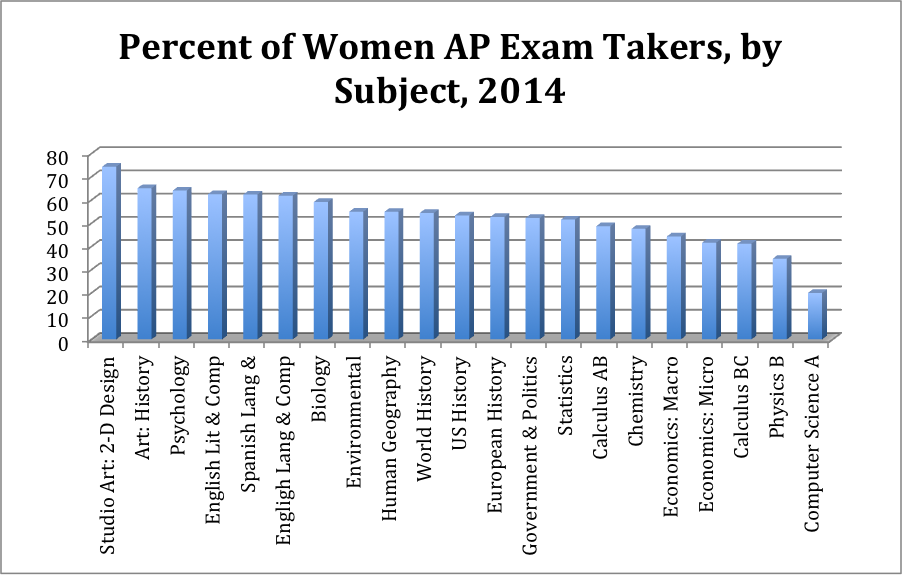
\includegraphics[width=\textwidth]{Percent-women-taking-AP-science-exams.png}
  \end{figure}
\end{frame}

\subsection{Who is a ``real programmer''?}

\begin{frame}{Who is a ``real programmer''?}
  For my first job as a software developer after leaving physics
  (1993): I found C very hard to learn

  \begin{itemize}
  \item Different levels of skill
  \item Different programming languages
  \item Different editor preferences
  \item Different application domains (front end, back end, etc.)
  \end{itemize}
\end{frame}

\subsection{First job}

\begin{frame}{Tech industry vs. academia}
  At first job (1993), noticed mockery of ``academic'' computer
  science:

  \begin{itemize}
  \item High-level languages were made fun of
  \item Memory management: garbage collection
  \item Safety
  \end{itemize}
\end{frame}

\begin{frame}{Engineering team vs. marketing, sales, management}
  ``Us vs. them'' mindset: caused a major project to eventually fail.

  \begin{itemize}
  \item As junior developer, didn't know what to say about what I saw
  \item I just kept reading the Dilbert comic strip
  \item No easy answers, but learned something for later
  \end{itemize}
\end{frame}

\subsection{Academia}

\begin{frame}{Brief time in academia (1997--1999)}
  Programming in C/C++ was very hard for me. I wanted to learn how to
  improve programming for everyone.

  \begin{block}{CMU CS PhD program}
    ``My career objective is to contribute to research into higher-level
    programming language concepts, their rigorous mathematical definition,
    implementations, and actual use in software development
    environments.''
  \end{block}

  \begin{itemize}
  \item My first time teaching (TA for freshman CS): a revelation
    about empathy!
  \item Lost interest in research
  \item Cared more about teaching, usability
  \item Academia a bad fit, I dropped out
  \end{itemize}

  Noticed mockery of industry (Java, attention to UI, etc.)
\end{frame}

\begin{frame}{Opportunities for empathy}
  \begin{alertblock}{Immersion in different communities}
    \begin{itemize}
    \item Observe what ``insiders'' think about the ``other''
    \item Actually swap roles
    \end{itemize}
  \end{alertblock}
\end{frame}

\begin{frame}{CMU psychology department (2002--present)}
  \begin{itemize}
  \item Boss is psychology professor
  \item My users: researchers in psychology, linguistics, law, etc.
  \item Older, nontechnical people
  \item Iterative process
  \end{itemize}

  Usability is critical:
  \begin{itemize}
  \item Error messages, recovery
  \item Git workflow
  \item Open communication about what software features are feasible
  \end{itemize}
\end{frame}


% Austin: sighted vs. blind

\section{Downsides of empathy?}

\begin{frame}{Downsides of empathy?}
  Power imbalances:
  \begin{itemize}
  \item Hard to have empathy for someone trying to destroy us
  \item Racists, sexists?
  \item Limited energy?
  \item Asymmetric situations: ``false equivalence''
  \end{itemize}

  \href{http://www.bostonreview.net/forum/paul-bloom-against-empathy}{Paul
    Bloom against empathy}: mostly focused on downsides of the emotional aspect
\end{frame}

\section{Some ongoing projects relevant to empathy}

\begin{frame}{Some ongoing projects relevant to empathy}
  \begin{itemize}
  \item My marriage
  \item Teaching chess
  \item Presentations for Code and Supply on Scala, Haskell, Rust
  \item New project in progress, to teach programming
  \item Ideas for improving usability for developers
  \item Contributing to open source projects
  \end{itemize}
\end{frame}


\section{Conclusion}

\subsection{Conclusion}

\begin{frame}{Conclusion}
  \begin{itemize}
    \item Empathy is part of being fully human
    \item Empathy is both affective and cognitive understanding
    \item Empathy is not always easy
    \item Expand your world, understand more people
    \item The tech world could use more empathy, especially for new
      learners, users
  \end{itemize}

  \href{http://radar.oreilly.com/2015/03/empathy-is-a-state-of-mind-not-a-specific-technique.html}{``Empathy
    is a state of mind, not a specific technique''}
\end{frame}

\appendix{Slides}

\begin{frame}{Slides}
  \begin{itemize}
  \item Source: \url{https://github.com/FranklinChen/empathy-talk}
  \item PDF with hyperlinks: \url{https://github.com/FranklinChen/empathy-talk/raw/master/presentation.pdf}
  \end{itemize}
\end{frame}

\end{document}


%%% Local Variables:
%%% mode: latex
%%% TeX-master: "presentation"
%%% End:
